\section{Session 2 - Digital circuit architecture}
\vspace{-15pt}\noindent\rule{\textwidth}{0.1pt}\vspace{-10pt}
    \subsection{Homework}
    \subsubsection{3.11 \textnormal{Analyze logic circuit}.}
    {\color{hwSolution}
        Truth Table:
        \begin{center}
            \begin{tabular}{c|c c}
                $A$ & $0$ & $1$ \\
                \hline
                $L$ & $1$ & $1$ \\
            \end{tabular}
            \[L = True\]
        \end{center}

        Wave Form ($t_{pd} = 50 ns$):
        \\
        \begin{center}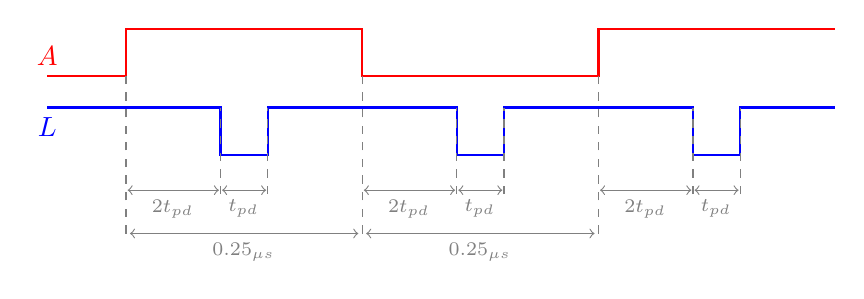
\begin{tikzpicture}
            \draw[red,thick]
                  (-1,1) node[above]{$A$}
                --(0.0,1.0)--(0.0,1.6)
                --(3.0,1.6)--(3.0,1.0)
                --(6.0,1.0)--(6.0,1.6)
                --(9.0,1.6);
            \draw[blue,thick]
                    (-1.0,0.6) node[below]{$L$}
                  --(1.2,0.6)--(1.2,0.0)
                  --(1.8,0.0)--(1.8,0.6)
                  --(4.2,0.6)--(4.2,0.0)
                  --(4.8,0.0)--(4.8,0.6)
                  --(7.2,0.6)--(7.2,0.0)
                  --(7.8,0.0)--(7.8,0.6)
                  --(9.0,0.6);
            \draw[dashed,gray]
                (0,-1.0)--(0,1.0) (1.2,-0.5)--(1.2,0.6) (1.8,-0.5)--(1.8,0.6)
                (3,-1.0)--(3,1.0) (4.2,-0.5)--(4.2,0.6) (4.8,-0.5)--(4.8,0.6)
                (6,-1.0)--(6,1.0) (7.2,-0.5)--(7.2,0.6) (7.8,-0.5)--(7.8,0.6);
            \draw[gray,<->]
                (0.02,-0.45)--(0.6,-0.45) node[below]{$_{2t_{pd}}$} --(1.18,-0.45);
            \draw[gray,<->]
                (1.22,-0.45)--(1.5,-0.45) node[below]{$_{t_{pd}}$} --(1.78,-0.45);
            \draw[gray,<->]
                (3.02,-0.45)--(3.6,-0.45) node[below]{$_{2t_{pd}}$} --(4.18,-0.45);
            \draw[gray,<->]
                (4.22,-0.45)--(4.5,-0.45) node[below]{$_{t_{pd}}$} --(4.78,-0.45);
            \draw[gray,<->]
                (6.02,-0.45)--(6.6,-0.45) node[below]{$_{2t_{pd}}$} --(7.18,-0.45);
            \draw[gray,<->]
                (7.22,-0.45)--(7.5,-0.45) node[below]{$_{t_{pd}}$} --(7.78,-0.45);
            \draw[gray,<->]
                (0.05,-1.00)--(1.5,-1.00) node[below]{$_{0.25_{\mu s}}$} --(2.95,-1.00);
            \draw[gray,<->]
                (3.05,-1.00)--(4.5,-1.00) node[below]{$_{0.25_{\mu s}}$} --(5.95,-1.00);
        \end{tikzpicture}\end{center}
    }
    
    \subsubsection{3.15 (c) \textnormal{Analyze logic circuit}.}
    {\color{hwSolution}
        At the case of \textit{$X\rightarrow HIGH$}:
        \[L = Z\]
        
        At the case of \textit{$X\rightarrow LOW$}: 
        \[L = A \overline{B}\]
    }
    
    \subsubsection{3.16 \textnormal{Pull or Push}.}
    {\color{hwSolution}
        应该选用$(a)$方案,因为74系列TTL可以接受的灌电流$(I_{OL}=16mA)$远大于高电平时的极限输出电流$(I_{OH}=-0.4mA)$,更适合驱动负载。且在本例中,考虑到$I_{LED}=10mA$,只有$I_{OL}$满足此条件。
    }
    
    \subsubsection{3.20 \textnormal{Mulityfunctional gate array}.}

    (1) Give the expression of Y (no simplification required):

    {\color{hwSolution}
        \[
            Y = \overline{E_3\,A\,B + E_2\,\bar{A}\,B + E_1\,A\,\bar{B} + E_0\,\bar{A}\,\bar{B}}
        \]
    }

    (2) Give the functionality of this circuit with $E_3\,E_2\,E_1\,E_0\,\rightarrow 0000 - 0111$:

    {\color{hwSolution}
        \begin{center}
            \begin{tabular}{c|l c l}
                $E$    & & $functionality$ & \\
                \hline
                $0~0~0~0$ & $Y = $ & $ True$ & 
                            \\
                $0~0~0~1$ & $Y = $ & $ \overline{\bar{A}\,\bar{B}}$ & 
                            $ = A + B$\\
                $0~0~1~0$ & $Y = $ & $ \overline{A\,\bar{B}} $ & 
                            $ = \bar{A} + B$\\
                $0~1~0~0$ & $Y = $ & $ \overline{\bar{A}\,B} $ & 
                            $ = A + \bar{B}$\\
                $0~0~1~1$ & $Y = $ & $ \overline{A\,\bar{B} + \bar{A}\,\bar{B}}$ & 
                            $ = B$\\
                $0~1~0~1$ & $Y = $ & $ \overline{\bar{A}\,B + \bar{A}\,\bar{B}}$ & 
                            $ = A$\\
                $0~1~1~0$ & $Y = $ & $ \overline{\bar{A}\,B + A\,\bar{B}}$ & 
                            $ = A\,B + \bar{A}\,\bar{B}$\\
                $0~1~1~1$ & $Y = $ & $ \overline{\bar{A}\,B + A\,\bar{B} + \bar{A}\,\bar{B}}$& 
                            $ = A\,B$\\
            \end{tabular}
        \end{center}
    }

    (2) Caculate the value range of R according to given conditions:
    
    {\color{hwSolution}
        First of all, we should be aware that there are AT MOST 2 Gates at LOW status. While ALL four gates may be at HIGH status.

        In case of 3 Highs and 1 Low, we get:
        \begin{equation*}
            \left\{\begin{array}{lcl}
                5V - R\cdot I_{CC} &<& 0.3V \\
                I_{CC} + 0.4mA \times 2 + 100\mu A \times 3 &<& 8 mA
            \end{array}
            \right.
        \end{equation*}

        In case of 4 Highs, we get:
        \begin{equation*}
            \left\{\begin{array}{lcl}
                5V - R\cdot I_{CC} &>& 3V \\
                I_{CC} + 100\mu A \times 4 &>& 20\mu A \times 2
            \end{array}
            \right.
        \end{equation*}

        Hence:
        \[
            R > 681\Omega
        \]
    }
